\chapter{Tests}
\label{chap:Tests}
The following chapter will describe the schedulability analysis made with UPPAAL, the unit tests and a functionality test made for the solution. 

\section{UPPAAL schedulability analysis}
\label{sec:UPPAAL schedulability}
As described in appendix \ref{chap:Increment three} section  \ref{sec:i3UPPAAL model}, Dumpsty contains three tasks: PrA, PrB and PrC. These three tasks all have individual WCET, which is not calculated, but rather tested, since calculating these through assembly code proved to be impossible due to unbound loops in libraries. After testing the individual tasks WCET, the worst case found would be significantly faster than what is labelled in UPPAAL, since the probability of hitting the actual worst case is close to impossible with the amount of tests done. In the following bulletpoints, all three tasks tested WCET and the WCET used in UPPAAL for the specific task is expressed, which is the first step to verify the schedulability of Dumpsty's tasks.


\begin{itemize}
	\item PrA \tab Tested: 1067 microseconds \tab UPPAAL: 2 milliseconds
	\item PrB \tab Tested: 732  microseconds \tab UPPAAL: 1 milliseconds
	\item PrC \tab	Tested: 8469 microseconds \tab UPPAAL: 9 milliseconds
\end{itemize}


For convenience, and to simplify the analysis, all tasks contain the worst case runtime of all interrupts and interrupt handlers that might occur during the execution of the task. These interrupts are generated by the motor encoders when Dumpsty is moving.


Figure \ref{UPPAAL Automata} depicts the automata created in UPPAAL from two declared classes. The first class, task PrA, is the cyclic executive instance for the task PrA. The second class is simply a CPU which is the key needed to run the task. Every task can grab the CPU, but only one may hold it at any given time. The CPU is then released when the task is done executing, and another task can then proceed to run.


\begin{figure}[h]
	\centering
	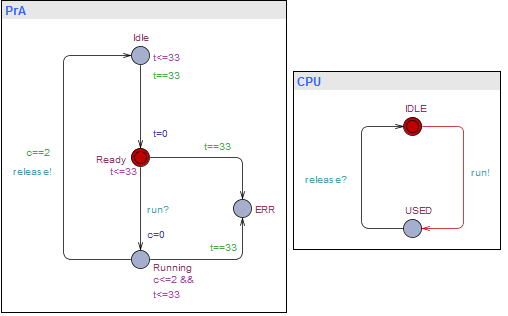
\includegraphics[scale=1]{billeder/UPPAALPr}
	\caption{Automata in UPPAAL}
	\label{UPPAAL Automata}
\end{figure}


In UPPAAL these automata might have more than one instance, defined by the amount of tasks declared. In this case, there are three instances of the first class:


\begin{itemize}
	\item PrA = TASK(1, 33, 2);
	\item PrB = TASK(2, 33, 1);
	\item PrC = TASK(3, 33, 9);
\end{itemize}


The integers declared for every task have different meanings. These integers will be explained by the case task PrA. In task PrA, the integer 1 is the ID for the task, 33 is the deadline for the task in milliseconds, and 2 is the worst-case execution time for the task. The deadline for all tasks are the same, since this is the minimal interarrival-time(MIT) for coordinates from the Kinect sensor. All code has to be executed within the MIT of these coordinates, since a new coordinate will alter the path the robot choose. 


The last step in the UPPAAL schedulability analysis is to use the verifier. This is done with two queries, found in listing \ref{Queries}. The first query checks if, after some amount of time, greater than zero, all tasks has been executed at least once and all tasks are in the ready state. The second query checks that no task ever hits an error-state. If these two queries both succeed, the tasks can all be executed within the deadline, and the schedulability analysis is successful, and in this case, with tasks PrA, PrB and PrC, the tasks are schedulable within the deadlines.


\begin{lstlisting}[caption={Queries for UPPAAL}, label={Queries}]
E<> PrA.Ready and PrB.Ready and PrC.Ready and PrA.t==0 and PrB.t==0 and PrC.t==0 and time>0
E[] not (PrA.ERR or PrB.ERR or PrC.ERR)
\end{lstlisting}


\section{Unit test}
\label{sec:Unit test}
To make the unit test on the arduino code, the library ArduinoUnit has been used \citep{au}. For the arduino code there has been conducted 12 unit tests, which have been split up into two different kind of unit tests, testing the two functions driveTowardsGoal() and updatePosAndHead(). \newline
The coordinates sent to Dumpsty in the unit tests are simulated, since this is the best representation of how the robot would work under perfect conditions. These unit tests reflect how Dumpsty performs in an environment with instantaneous received data from a sensor with great precision, where the sensor will send new data every 33ms. 
The first type will test the function driveTowardsGoal() and has 3 different inputs being starting position, goal position and the heading of the robot. The robot will start at its starting position with the given heading, and will then have to move towards the goal position. In the description of the test, if no heading is described, the heading is 0. For a code near perspective of this unit test type, check listing \ref{ut1}.


\begin{lstlisting}[caption={First type of Unit test}, label={ut1}]
test(curPos30\_150goalPos30\_150Head1){
heading = itok(1);
posX = itok(30);
posY = itok(150);
goalX = itok(30);
goalY = itok(150);
String result = driveTowardsGoal();
assertEqual(result, "goal");
}
\end{lstlisting}


The second type of unit test will test the function updatePosAndHead(). The test takes 4 inputs being the starting position, the heading, millimetres to move on the right motor and millimetres to move on the left motor. The robot will start at its starting position with the given heading, and will move the given millimetres for each motor. Then the unit test will check if the robot is within 0.01mm of the asserted position. An example of this type of unit test can been found in listing \ref{ut2}.


\begin{lstlisting}[caption={Second type of Unit test}, label={ut2}]
test(pos300_250Head075Left12Right5){
heading = ftok(0.75);
posX = itok(300);
posY = itok(250);
rightTotal = 5;
rightTemp = 0;
leftTotal = 12;
leftTemp = 0;


updatePosAndHead();


assertMore(posX, ftok(302.826));
assertLess(posX, ftok(302.836)); 


assertMore(posY, ftok(253.034));
assertLess(posY, ftok(253.044));


assertMore(heading, ftok(0.717));
assertLess(heading, ftok(0.727));  
}
\end{lstlisting}


Table \ref{table:Unit tests} includes all the unit tests made for the arduino code. The table consists of a description of the unit test and if the test passed or failed. 
\begin{table}[H]
	\begin{center}
		\begin{tabular}{ | p{10cm} | p{5cm} |}
			\hline
			\textbf{Test description} & \textbf{Result} \\ \hline	
			The robot is at position (30, 150), and gets the same coordinate sent, this will check if the robot says it is at goal or will try move to a new position. & Passed \\ \hline
			The robot will have a starting position at (0, 0) and will be given a new coordinate at (0, 150), the robot should then drive forward in a straight line. & \textcolor{red}{Failed} \\ \hline
			The robot will start at position (0, 0) with a heading of (1) and will be given the new coordinate (0, -150) which should make the robot turn left.  & Passed \\ \hline
			The robots starting position is (150, 150) with a heading of (-1) and is given a new coordinate at (140, 100). This means the robot will be pointing towards the top right and will have to drive down towards the right. & \textcolor{red}{Failed} \\ \hline
			The robot starts in position (150, 150) with a heading of (-1) making the robot point towards the top right. The robot is then given a new coordinate (300, 200), the robot should then turn around it self and move towards the top left & Passed \\ \hline
			The robots starting position is (0, 0) with a heading of (1), making the robot point towards the top left. The robot is given a new coordiante (0, 300). The robot will only use one motor till its heading is 0, and then drive forwards to the new coordinate  & Passed \\ \hline
			The robots starting position is (0, 0) and is given the new coordinate (-150, 300). The robot should the move towards the new position at the top right. & Passed \\ \hline
			The robot has the starting position (300, 250) with a heading of (0.75). The robot is ordered to drive 5mm with the right motor, and 12mm with the left motor and check if the new position is within a precision of 0.01mm of the asserted position. & Passed \\ \hline
			The robot has the starting position (160, 100) with a heading of (-0.4) and is to drive 14mm with the right motor and 3mm with the left motor. The robot should be within 0.01mm of the asserted position & Passed \\ \hline
			The robot is at starting position (120, 200) with a heading of (1). The robot is to drive 10mm with each motor, and be within 0.01mm of the asserted position & Passed \\ \hline
			The robot has the starting position (0, 0) and the robot is to drive 10mm with the right motor. The robot should be within 0.01mm of thte asserted position & Passed \\ \hline
			The robot has the starting position (0, 0) and the robot is to drive 10mm with the left motor. The robot should be within 0.01mm of thte asserted position & Passed \\ \hline
		\end{tabular}
		\caption{Table of conducted unit tests}
		\label{table:Unit tests}
	\end{center}
\end{table}


All the failed test have been corrected and is now working as expected. 


\section{Functional test}
\label{sec:LasseSucks}
Now that the unit tests for Dumpsty are successful, the functionality of Dumpsty must be tested as well. This is done through a functional test, where Dumpsty is placed in an appropriate environment, and then the entire system will be tested. This is done through throwing an object in front of the Kinect sensor, having the Kinect print the sent coordinates, and having the robot moving to the point. The actual impact point of the object will also be marked on the ground, and the distance between all three points will be measured in cm, shown in table \ref{table:FuncTest}. \newline
The three columns depicts the following:\newline
Predicted to impact: The distance from the predicted coordinate from the Kinect, to the actual impact point of the object.\newline
Predicted to robot: The distance from the predicted coordinate to the robot, after the robot has stopped moving.\newline
Robot to impact: The distance from the robot after it has stopped moving, to the actual impact point of the object.


\begin{table}[H]
	\begin{center}
		\begin{tabular}{ | p{5cm} | p{5cm} | p{5cm} |}
			\hline
			\textbf{Predicted to impact} & \textbf{Predicted to robot} & \textbf{Robot to impact} \\ \hline
			23 & 11 & 34 \\ \hline
			11.5 & 6.5 & 14 \\ \hline
			19.5 & 8 & 26 \\ \hline
			19 & 10.5 & 26.5 \\ \hline
			36 & 8.5 & 43.5 \\ \hline
			48 & 11 & 56 \\ \hline
			9.5 & 11 & 21 \\ \hline
			16 & 5.5 & 11 \\ \hline
			49.5 & 11 & 48.5 \\ \hline
			13 & 11 & 19 \\ \hline
			
		\end{tabular}
		\caption{Table of conducted functional tests}
		\label{table:FuncTest}
	\end{center}
\end{table}


\section{Summary}
\label{sec:summary}
The scheduling is rather simple since the tasks are small and the platform to perform the tasks is faster and has more memory than needed, as shown in the schedulability analysis. The unit tests are implying that the robot should be working as intended, since it passed most of the tests and the tests which failed were corrected. The functionality test shows that the Kinect didn’t correctly predict where the impact point of the object is, and the robot doesn’t stop at the exact coordinate point sent by the Kinect. 


As one can see, Dumpsty is consistently close to 10 cm from the predicted coordinates, which could be caused by the servo motors drift after the motors has been released in the code. The fact that the prediction has a range of misprediction of 10 - 50 cm is either due to miscalculations in the Kinect code, or the Kinect having hardware issues, creating a distorted depth-picture.






